\documentclass{sbc2023}%

\usepackage{graphicx}
\usepackage[misc,geometry]{ifsym}
\usepackage{fontspec}
\usepackage{fontawesome}
\usepackage{academicons}
\usepackage{color}
\usepackage{hyperref}
\usepackage{aas_macros}
\usepackage[bottom]{footmisc}
\usepackage{supertabular}
\usepackage{afterpage}
\usepackage{url}
\usepackage{pifont}
\usepackage{multicol}
\usepackage{multirow}

\setcitestyle{square}

\definecolor{orcidlogo}{rgb}{0.37,0.48,0.13}
\definecolor{unilogo}{rgb}{0.16, 0.26, 0.58}
\definecolor{maillogo}{rgb}{0.58, 0.16, 0.26}
\definecolor{darkblue}{rgb}{0.0,0.0,0.0}
\hypersetup{colorlinks,breaklinks,
            linkcolor=darkblue,urlcolor=darkblue,
            anchorcolor=darkblue,citecolor=darkblue}

\jid{JBCS}
\jtitle{Arquitetura de Computadores --- Trabalho Prático 3, 2026}
\doi{}
\copyrightstatement{Trabalho acadêmico --- Arquitetura de Computadores}
\jyear{2026}

\title[Otimização Paralela de GEMM]{Otimização Paralela de Multiplicação de Matrizes Densas (GEMM) em CPU e GPU}

% ===================================================================
% TODO: substitua pelos nomes/ORCID/instituição do seu grupo.
% ===================================================================
\author[Grupo 202X]{
\affil{\textbf{Nome do(a) Aluno(a) 1}~\textcolor{blue}{\faEnvelopeO}~~[~\textbf{Instituição}~|\href{mailto:email@dominio}{~\textbf{\textit{email@dominio}}}~]}

\affil{\textbf{Nome do(a) Aluno(a) 2}~~[~\textbf{Instituição}~|\href{mailto:email@dominio}{~\textbf{\textit{email@dominio}}}~]}
}

\begin{document}

\begin{frontmatter}
\maketitle

\begin{mail}
Disciplina de Arquitetura de Computadores --- Trabalho Prático 3: Processamento paralelo em CPU e GPU.
\end{mail}

\begin{dates}
\small{\textbf{Ambiente:} Google Colab~~~$\bullet$~~~\textbf{CPU:} Intel Xeon @ 2.00\,GHz (2 vCPUs)~~~$\bullet$~~~\textbf{GPU:} NVIDIA Tesla T4}
\end{dates}

\begin{abstract}
\textbf{Abstract.~}
\noindent Este trabalho parte de uma implementação ingênua da multiplicação de matrizes densas (GEMM, $C = A \times B$) e a evolui através de cinco otimizações cumulativas: melhoria de localidade de memória por transposição, blocagem/\textit{tiling}, vetorização SIMD automática, paralelismo de memória compartilhada com OpenMP e aceleração em GPU com CUDA (versões \textit{naïve} e \textit{tiled} com memória compartilhada). Todas as versões foram validadas contra a referência sequencial (erro absoluto máximo $\leq 9{,}2\times10^{-5}$, compatível com a reordenação de somas em ponto flutuante de 32 bits) e cada experimento foi repetido 5 vezes, reportando-se a média. Em CPU, a transposição de $B$ dobrou o desempenho ($1{,}97\times$) e a blocagem com $BS=64$ atingiu $13{,}5$ GFLOP/s ($20{,}6\times$ sobre a versão ingênua) para $N=512$. Em GPU, o kernel \textit{tiled} alcançou $750$ GFLOP/s ($N=512$), cerca de $1142\times$ o tempo do kernel da CPU ingênua. Discute-se ainda o impacto das cópias \textit{host}--\textit{device}, a baixa escalabilidade do OpenMP no ambiente de 2 vCPUs do Colab e os cuidados metodológicos necessários nesse tipo de plataforma compartilhada.
\end{abstract}

\begin{keywords}
GEMM, Vetorização SIMD, OpenMP, CUDA, Localidade de cache, Desempenho
\end{keywords}

\end{frontmatter}


\section{Introdução}
\label{sec:intro}

A multiplicação de matrizes densas (\textit{General Matrix Multiply} --- GEMM) é uma das operações mais estudadas em computação de alto desempenho, por ser ao mesmo tempo conceitualmente simples e fortemente limitada pela hierarquia de memória. Para matrizes quadradas $N \times N$, o número de operações de ponto flutuante é aproximadamente $2N^3$, e o desempenho é medido em
\begin{equation}\label{eq:gflops}
\text{GFLOP/s} = \frac{2N^3}{t \times 10^{9}},
\end{equation}
onde $t$ é o tempo médio de execução em segundos.

O objetivo deste trabalho é partir de uma implementação ingênua e medir, de forma controlada, o ganho proporcionado por cada técnica de otimização: (i) localidade de memória via transposição de $B$; (ii) blocagem/\textit{tiling}; (iii) vetorização SIMD automática pelo compilador; (iv) paralelismo com OpenMP; e (v) aceleração em GPU com CUDA. Além de quantificar tempo, GFLOP/s, \textit{speedup} e eficiência, busca-se uma análise crítica das limitações observadas --- em especial as impostas pelo ambiente compartilhado do Google Colab. Conforme exigido, nenhuma biblioteca de álgebra linear pronta (BLAS, cuBLAS, Eigen) foi utilizada na parte principal.

\subsection{Definições de métricas}

Adotam-se as seguintes definições. O \textbf{\textit{speedup}} de uma versão em relação à referência ingênua sequencial é $S = t_{\text{naive}} / t_{\text{versão}}$, de modo que a versão ingênua tem $S = 1{,}0$. Para as versões paralelas, define-se ainda a \textbf{eficiência paralela} $E = S_p / p$, onde $S_p = t_{1}/t_{p}$ é o \textit{speedup} de escalabilidade forte do \emph{próprio} algoritmo OpenMP (tempo com 1 \textit{thread} sobre o tempo com $p$ \textit{threads}). Essa separação é importante porque o \textit{speedup} sobre a ingênua mistura três efeitos distintos (ordem de laços, vetorização e paralelismo), enquanto a eficiência isola o ganho de paralelismo.


\section{Metodologia Experimental}
\label{sec:metodo}

\subsection{Ambiente de execução}

Todos os experimentos foram executados no Google Colab. As características de \textit{hardware} e \textit{software} relevantes, coletadas por \texttt{lscpu}, \texttt{nvidia-smi} e pelos compiladores, estão na Tabela~\ref{tab:ambiente}. Destaca-se que a CPU disponível expõe apenas \textbf{2 vCPUs} correspondentes a \textbf{1 núcleo físico com 2 \textit{threads}} (\textit{hyper-threading}), fato determinante para a análise de escalabilidade da Seção~\ref{sec:openmp}.

\begin{table}[!ht]
\caption{Ambiente experimental (Google Colab).}
\centering
\begin{tabular}{@{}ll@{}}
\hline\hline
Componente & Especificação \\
\hline
CPU & Intel Xeon @ 2.00\,GHz \\
vCPUs / núcleos & 2 \textit{threads} / 1 núcleo físico (HT) \\
Cache L1d / L2 / L3 & 32\,KiB / 1\,MiB / 38{,}5\,MiB \\
ISA SIMD & SSE, AVX2, AVX-512 (F/DQ/CD/BW/VL) \\
GPU & NVIDIA Tesla T4 (15\,GB, Turing) \\
Compilador C & gcc 11.4.0 (Ubuntu 22.04) \\
Compilador CUDA & nvcc 12.8 \\
\hline\hline
\end{tabular}
\label{tab:ambiente}
\end{table}

\subsection{Implementações}

O programa em C contém cinco versões de CPU. A versão \texttt{naive} usa a ordem clássica de laços $i$--$j$--$k$, em que o laço interno percorre $B$ por colunas (passo $N$). A versão \texttt{transposed} pré-transpõe $B$ em $B^{T}$, tornando o produto interno um percurso sequencial de duas linhas contíguas. As versões \texttt{blocked} e \texttt{blocked\_openmp} aplicam blocagem $BS \times BS$ com núcleo na ordem $i$--$k$--$j$ (laço interno contíguo e vetorizável). As versões \texttt{openmp} e \texttt{blocked\_openmp} paralelizam com \texttt{\#pragma omp parallel for} sobre as linhas/blocos de linhas de $C$ (escritas em linhas disjuntas, sem condição de corrida). A compilação usou \texttt{-O3 -march=native -fopenmp}, ativando a vetorização automática.

Em CUDA, a versão \texttt{cuda\_naive} atribui uma \textit{thread} por elemento de $C$, e a versão \texttt{cuda\_tiled} usa memória compartilhada com blocos $\texttt{TILE}=16$, carregando colaborativamente \textit{tiles} de $A$ e $B$ para reduzir acessos à memória global.

\subsection{Protocolo de medição}

Cada configuração foi executada $5$ vezes; reporta-se o \textbf{tempo médio}. Na CPU o tempo é obtido com \texttt{clock\_gettime(CLOCK\_MONOTONIC)} em torno do \textit{kernel} de cálculo; na GPU, com \texttt{cudaEvent}, medindo \emph{separadamente} a cópia \textit{host}$\rightarrow$\textit{device} (H2D), a execução do \textit{kernel} e a cópia \textit{device}$\rightarrow$\textit{host} (D2H). Os tamanhos testados foram $N \in \{128, 256, 512\}$ na CPU e $N \in \{128, 256, 512, 1024\}$ na GPU; os blocos $BS \in \{16, 32, 64\}$; e as contagens de \textit{threads} $\{1, 2, 4, 8\}$. Todas as versões foram validadas pelo erro absoluto máximo contra a referência \texttt{gemm\_naive}.

\subsection{Correção e validação}

Todas as versões produziram resultados corretos. O erro absoluto máximo permaneceu nulo ou da ordem de $10^{-5}$ ($\leq 4{,}6\times10^{-5}$ para $N=512$ na CPU e $\leq 9{,}2\times10^{-5}$ para $N=1024$ na GPU). Esses desvios são consequência esperada da \emph{reordenação} das somas em ponto flutuante de precisão simples (as versões otimizadas acumulam em ordem diferente da referência), não de erro algorítmico, e crescem linearmente com $N$, como previsto pela análise de erro de acumulação.


\section{Resultados em CPU}
\label{sec:cpu}

A Tabela~\ref{tab:cpu} consolida os tempos médios e o desempenho das versões de CPU. A Figura~\ref{fig:cpu_gflops} compara as famílias de versões nos três tamanhos.

\begin{table}[!ht]
\caption{Resultados em CPU (média de 5 execuções). Tempo em segundos.}
\centering
\small
\begin{tabular}{@{}llrrr@{}}
\hline\hline
Versão & Config. & $N$ & Tempo (s) & GFLOP/s \\
\hline
naive          & ---        & 128 & 0,002873 & 1,46 \\
transposed     & ---        & 128 & 0,001909 & 2,20 \\
blocked        & $BS{=}64$  & 128 & 0,000227 & 18,46 \\
openmp         & 8 \textit{thr} & 128 & 0,000343 & 12,23 \\
\hline
naive          & ---        & 256 & 0,020810 & 1,61 \\
transposed     & ---        & 256 & 0,018397 & 1,82 \\
blocked        & $BS{=}64$  & 256 & 0,003626 & 9,25 \\
openmp         & 8 \textit{thr} & 256 & 0,002585 & 12,98 \\
\hline
naive          & ---        & 512 & 0,408878 & 0,66 \\
transposed     & ---        & 512 & 0,207847 & 1,29 \\
blocked        & $BS{=}16$  & 512 & 0,034401 & 7,80 \\
blocked        & $BS{=}32$  & 512 & 0,027339 & 9,82 \\
blocked        & $BS{=}64$  & 512 & 0,019870 & 13,51 \\
openmp         & 1 \textit{thr} & 512 & 0,023963 & 11,20 \\
openmp         & 2 \textit{thr} & 512 & 0,025058 & 10,71 \\
openmp         & 4 \textit{thr} & 512 & 0,024120 & 11,13 \\
openmp         & 8 \textit{thr} & 512 & 0,012476 & 21,52 \\
blocked\_openmp & 4 \textit{thr} & 512 & 0,019248 & 13,95 \\
\hline\hline
\end{tabular}
\label{tab:cpu}
\end{table}

\begin{figure}[!ht]
\begin{center}
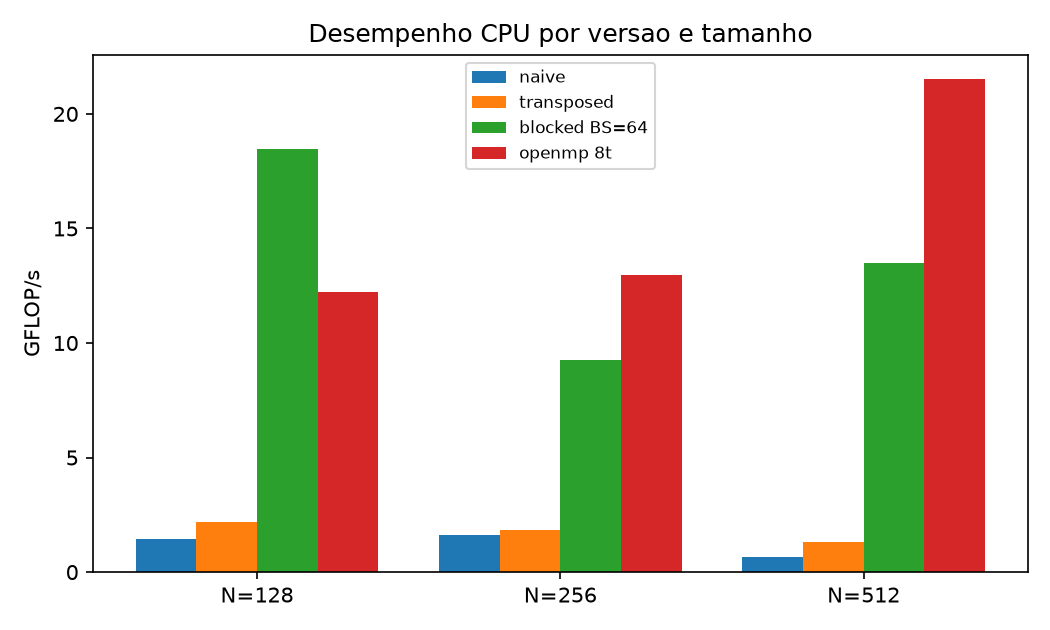
\includegraphics[width=\columnwidth]{figs/cpu_gflops.png}
\caption{Desempenho (GFLOP/s) das principais versões de CPU para $N \in \{128,256,512\}$.}
\label{fig:cpu_gflops}
\end{center}
\end{figure}

\subsection{Localidade e transposição}

A versão ingênua é a mais lenta em todos os tamanhos, atingindo apenas $0{,}66$ GFLOP/s para $N=512$ --- menos de $1\%$ do pico teórico da máquina. A transposição de $B$ reduziu o tempo de $0{,}409$\,s para $0{,}208$\,s ($N=512$), um \textit{speedup} de $1{,}97\times$. O ganho é real, porém modesto: embora a transposição torne o acesso a $B^{T}$ sequencial e vetorizável, o algoritmo ainda relê uma linha inteira de $B^{T}$ por elemento de saída, com baixa reutilização, permanecendo limitado pela largura de banda de memória.

\subsection{Blocagem e tamanho de bloco}

A blocagem foi a otimização \emph{serial} mais eficaz: para $N=512$, o desempenho saltou para $13{,}5$ GFLOP/s ($20{,}6\times$ sobre a ingênua). A Figura~\ref{fig:blocksize} mostra que, dentro da faixa testada, \textbf{$BS=64$ foi consistentemente o melhor} ($7{,}80 \to 9{,}82 \to 13{,}51$ GFLOP/s à medida que $BS$ cresce de $16$ para $64$). Um bloco $64\times64$ de \texttt{float} ocupa $16$\,KiB; os três \textit{tiles} ativos ($\approx 48$\,KiB) ainda cabem confortavelmente no cache L2 de 1\,MiB, maximizando a reutilização e amortizando o custo dos laços, enquanto blocos menores desperdiçam linhas de cache e adicionam sobrecarga de controle.

\begin{figure}[!ht]
\begin{center}
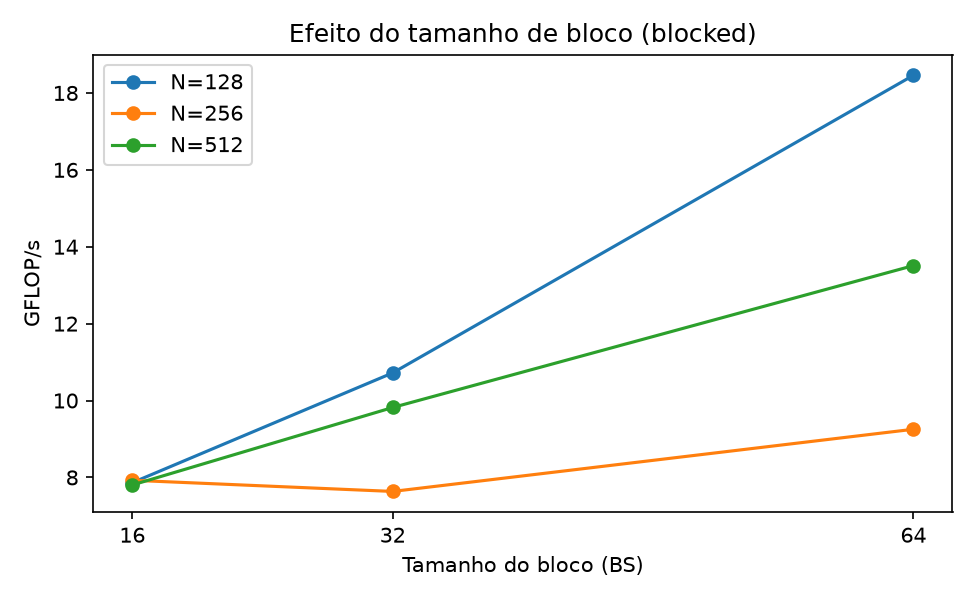
\includegraphics[width=\columnwidth]{figs/cpu_blocksize.png}
\caption{Efeito do tamanho de bloco $BS$ no desempenho da versão \texttt{blocked}.}
\label{fig:blocksize}
\end{center}
\end{figure}

\subsection{Vetorização SIMD}

O relatório de vetorização (\texttt{-fopt-info-vec-optimized}) confirma que o compilador \textbf{vetorizou os laços internos das quatro versões otimizadas} usando vetores de 32 \textit{bytes} (AVX2, 8 \texttt{float} por instrução), com mensagens como \texttt{``loop vectorized using 32 byte vectors''} nas linhas correspondentes a \texttt{gemm\_transposed}, \texttt{gemm\_blocked}, \texttt{gemm\_openmp} e \texttt{gemm\_blocked\_openmp}. O laço interno da versão \texttt{naive}, por ser uma redução com acesso a $B$ por coluna (passo $N$), \emph{não} aparece como vetorizado --- evidência direta de que a má localidade impede o aproveitamento das unidades SIMD. Vários laços foram ``versionados por possível \textit{aliasing}'', indicando que o compilador gerou caminhos vetorizados e escalares decididos em tempo de execução.

\subsection{Paralelismo OpenMP}
\label{sec:openmp}

A Figura~\ref{fig:openmp} mostra a escalabilidade do OpenMP. Os resultados \emph{não} se aproximam do ideal: para $N=512$, passar de 1 para 2 \textit{threads} \textbf{não} trouxe ganho ($t_1 = 0{,}0240$\,s vs.\ $t_2 = 0{,}0251$\,s; $S_2 = 0{,}96$, $E_2 = 0{,}48$), e com 4 \textit{threads} a eficiência cai para $0{,}25$. A explicação principal está na Tabela~\ref{tab:ambiente}: o Colab oferece \textbf{apenas 1 núcleo físico} (2 \textit{threads} lógicas por \textit{hyper-threading}). Não há paralelismo real de execução para além de um núcleo, e o problema já é limitado por largura de banda de memória. O valor anômalo de $21{,}5$ GFLOP/s com 8 \textit{threads} ($S=32{,}8\times$ sobre a ingênua) deve ser interpretado com cautela: trata-se muito provavelmente de variância do ambiente compartilhado (note-se também $t_2 > t_1$, fisicamente improvável em escalabilidade verdadeira), e não de ganho determinístico de paralelismo.

\begin{figure}[!ht]
\begin{center}
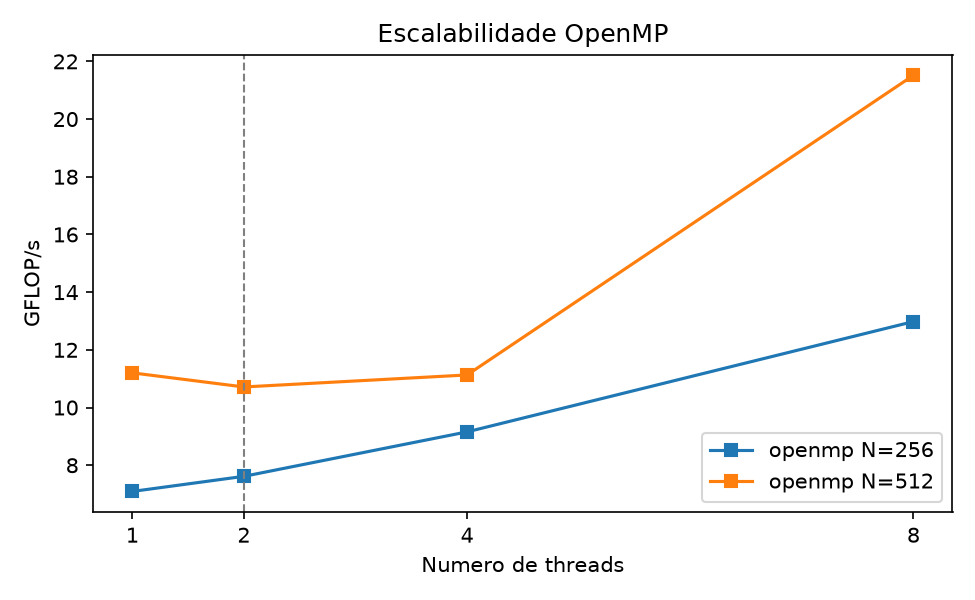
\includegraphics[width=\columnwidth]{figs/openmp_scaling.png}
\caption{Escalabilidade do OpenMP (GFLOP/s vs.\ número de \textit{threads}). A linha tracejada marca o limite de 2 vCPUs físicas.}
\label{fig:openmp}
\end{center}
\end{figure}


\section{Resultados em GPU}
\label{sec:gpu}

A Tabela~\ref{tab:gpu} apresenta os tempos da GPU, decompostos em H2D, \textit{kernel} e D2H. A Figura~\ref{fig:gpu_kernel} compara o desempenho dos \textit{kernels} e a Figura~\ref{fig:gpu_breakdown} mostra a composição do tempo total.

\begin{table*}[!ht]
\caption{Resultados em GPU (Tesla T4, média de 5 execuções). Tempos em milissegundos.}
\centering
\begin{tabular*}{\textwidth}{@{}l\x c\x c\x c\x c\x c\x c\x c@{}}
\hline\hline
Versão & $N$ & H2D (ms) & \textit{kernel} (ms) & D2H (ms) & total (ms) & \textit{kernel} GFLOP/s & total GFLOP/s \\
\hline
cuda\_naive & 128  & 0,210 & 20,571$^\dagger$ & 0,040 & 20,820 & 0,2$^\dagger$ & 0,2$^\dagger$ \\
cuda\_tiled & 128  & 0,071 & 0,064 & 0,037 & 0,171 & 65,95 & 24,51 \\
cuda\_naive & 256  & 0,174 & 0,124 & 0,114 & 0,411 & 270,66 & 81,61 \\
cuda\_tiled & 256  & 0,174 & 0,092 & 0,131 & 0,398 & 363,84 & 84,37 \\
cuda\_naive & 512  & 0,643 & 0,569 & 0,438 & 1,650 & 471,38 & 162,64 \\
cuda\_tiled & 512  & 0,633 & 0,358 & 0,409 & 1,399 & 750,05 & 191,82 \\
cuda\_naive & 1024 & 2,116 & 5,392 & 1,587 & 9,095 & 398,26 & 236,11 \\
cuda\_tiled & 1024 & 1,984 & 5,707 & 1,427 & 9,119 & 376,30 & 235,51 \\
\hline\hline
\end{tabular*}
\\[2pt]
{\footnotesize $^\dagger$ Primeiro \textit{kernel} lançado na sessão: o valor de 20,6\,ms é um artefato de inicialização do contexto/JIT da CUDA e foi desconsiderado na análise.}
\label{tab:gpu}
\end{table*}

\begin{figure}[!ht]
\begin{center}
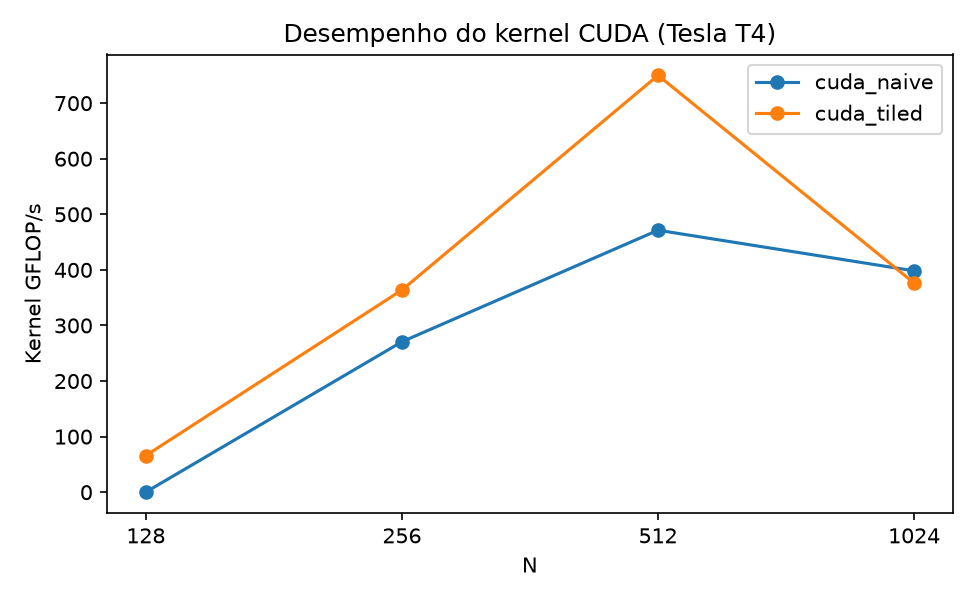
\includegraphics[width=\columnwidth]{figs/gpu_kernel_gflops.png}
\caption{Desempenho do \textit{kernel} CUDA (GFLOP/s) para \texttt{naive} e \texttt{tiled}.}
\label{fig:gpu_kernel}
\end{center}
\end{figure}

\begin{figure}[!ht]
\begin{center}
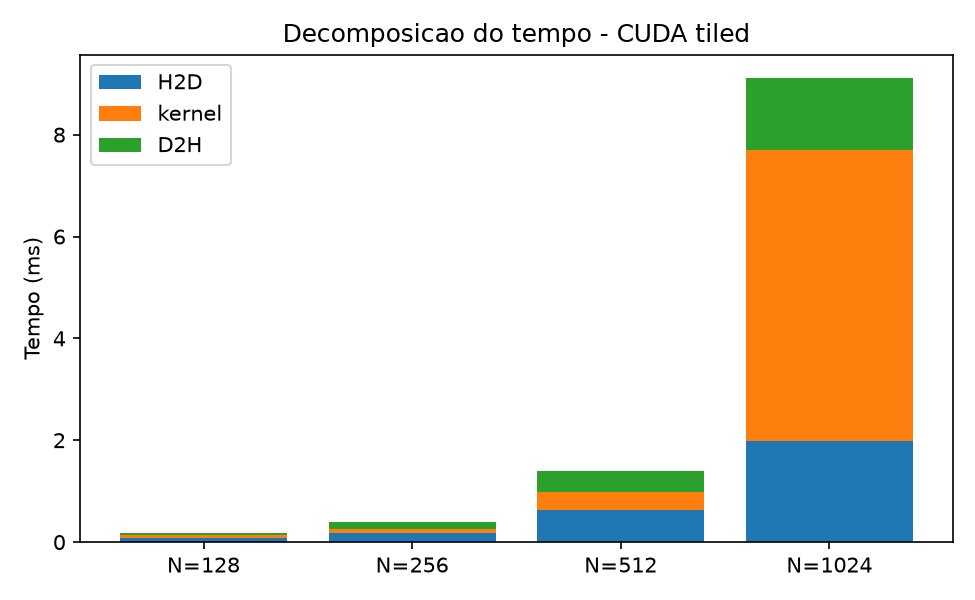
\includegraphics[width=\columnwidth]{figs/gpu_breakdown.png}
\caption{Decomposição do tempo total da versão \texttt{cuda\_tiled} em cópias (H2D, D2H) e \textit{kernel}.}
\label{fig:gpu_breakdown}
\end{center}
\end{figure}

\subsection{Kernel vs.\ tempo total}

Considerando \emph{apenas o kernel}, a GPU é ordens de grandeza mais rápida que a CPU. Para $N=512$, o \textit{kernel} \texttt{tiled} atinge $750$ GFLOP/s, contra $\approx 21{,}5$ GFLOP/s da melhor CPU --- e $\approx 1142\times$ o tempo do \textit{kernel} da CPU ingênua. O uso de memória compartilhada teve impacto claro nos tamanhos intermediários: em $N=512$, o \textit{tiled} é $1{,}59\times$ mais rápido que o \texttt{naive} ($0{,}358$\,ms vs.\ $0{,}569$\,ms).

Há, porém, duas nuances. Primeiro, ao se incluir as cópias, o desempenho ``efetivo'' (\textit{total} GFLOP/s) cai drasticamente para tamanhos pequenos: em $N=128$, o \textit{tiled} rende $66$ GFLOP/s no \textit{kernel} mas apenas $24{,}5$ GFLOP/s no total, pois as transferências PCIe e a latência de lançamento dominam (Figura~\ref{fig:gpu_breakdown}). Segundo, em $N=1024$ a vantagem do \textit{tiled} desaparece ($376$ vs.\ $398$ GFLOP/s): com \texttt{TILE}=16, o \textit{kernel} ingênuo já se beneficia bastante dos caches L1/L2 da arquitetura Turing, e ambos convergem para a faixa limitada pela largura de banda da memória global do dispositivo.


\section{Comparação Consolidada}
\label{sec:comparacao}

A Tabela~\ref{tab:final} consolida a comparação para $N=512$ (maior tamanho comum a CPU e GPU). Os \textit{speedups} são calculados em relação ao tempo da CPU ingênua ($t_{\text{naive}}=0{,}409$\,s); para as versões CUDA usa-se o tempo do \textit{kernel}. A eficiência é reportada apenas para as versões paralelas OpenMP (escalabilidade forte sobre 1 \textit{thread}).

\begin{table*}[!ht]
\caption{Tabela final de comparação para $N=512$.}
\centering
\begin{tabular*}{\textwidth}{@{}l\x c\x c\x c\x c\x c\x l@{}}
\hline\hline
Versão & $N$ & Tempo médio & GFLOP/s & \textit{Speedup} & Eficiência & Observações \\
\hline
CPU naive            & 512 & 0,408878\,s & 0,66   & 1,0    & 1,0   & Referência \\
CPU transposed       & 512 & 0,207847\,s & 1,29   & 1,97   & ---   & Localidade \\
CPU blocked ($BS{=}64$) & 512 & 0,019870\,s & 13,51  & 20,58  & ---   & Cache \\
CPU OpenMP 2 \textit{threads} & 512 & 0,025058\,s & 10,71  & 16,32  & 0,48  & \textit{Threads} \\
CPU OpenMP 4 \textit{threads} & 512 & 0,024120\,s & 11,13  & 16,95  & 0,25  & \textit{Threads} \\
CUDA naive           & 512 & 0,569\,ms (\textit{kernel}) & 471,38 & 718    & ---   & Kernel simples \\
CUDA tiled           & 512 & 0,358\,ms (\textit{kernel}) & 750,05 & 1142   & ---   & Mem.\ compartilhada \\
\hline\hline
\end{tabular*}
\label{tab:final}
\end{table*}

Para referência, considerando o \emph{tempo total} (com cópias), a versão \texttt{cuda\_tiled} mantém \textit{speedup} de $292\times$ e a \texttt{cuda\_naive} de $248\times$ sobre a CPU ingênua, evidenciando que mesmo com a sobrecarga de comunicação a GPU permanece muito superior para este tamanho.


\section{Discussão}
\label{sec:discussao}

Esta seção responde diretamente às questões propostas no enunciado.

\paragraph{1. Por que a versão ingênua tem baixo desempenho?}
Porque seu laço interno percorre $B$ por coluna (\texttt{B[k*N+j]}, passo $N$), gerando uma falha de cache a cada acesso e nenhuma reutilização de dados. Além disso, a redução com acesso \textit{strided} impede a vetorização. O resultado é uma operação totalmente limitada pela latência de memória --- $0{,}66$ GFLOP/s para $N=512$.

\paragraph{2. O impacto da transposição de $B$ foi significativo?}
Foi positivo, porém moderado: $1{,}97\times$ ($N=512$). Tornar o acesso a $B^{T}$ sequencial habilita a vetorização SIMD e melhora a localidade espacial, mas o algoritmo continua relendo dados sem blocagem, permanecendo limitado por largura de banda --- por isso o ganho é muito menor que o da blocagem.

\paragraph{3. Qual tamanho de bloco foi melhor?}
$BS=64$, em todos os tamanhos. Blocos maiores aumentam a reutilização de dados que cabem no cache (um \textit{tile} $64\times64$ de \texttt{float} ocupa $16$\,KiB; o conjunto de trabalho cabe no L2 de 1\,MiB) e amortizam a sobrecarga dos laços, enquanto blocos de $16$ subutilizam as linhas de cache.

\paragraph{4. O compilador vetorizou o código?}
Sim. O relatório \texttt{-fopt-info-vec-optimized} reporta ``\texttt{loop vectorized using 32 byte vectors}'' (AVX2) para os laços internos de \texttt{transposed}, \texttt{blocked}, \texttt{openmp} e \texttt{blocked\_openmp}. A versão \texttt{naive} não aparece vetorizada, confirmando que a má localidade bloqueia o uso das unidades SIMD.

\paragraph{5. O \textit{speedup} com OpenMP foi próximo do ideal?}
Não. Com 2 \textit{threads}, $S_2 = 0{,}96$ ($E_2 = 0{,}48$) --- praticamente nenhum ganho. A causa é estrutural: o Colab fornece apenas \textbf{1 núcleo físico} (2 \textit{threads} lógicas por \textit{hyper-threading}), e o problema é limitado por banda de memória. Não há recursos de execução para um \textit{speedup} próximo de 2.

\paragraph{6. A eficiência diminuiu com mais \textit{threads}?}
Sim, monotonicamente: $E_2 = 0{,}48 \to E_4 = 0{,}25 \to E_8 = 0{,}24$. Acima de 2 \textit{threads} há \textit{oversubscription} (mais \textit{threads} que vCPUs), com troca de contexto e contenção de memória, sem qualquer núcleo adicional para absorver o trabalho.

\paragraph{7. A GPU foi mais rápida considerando apenas o \textit{kernel}?}
Sim, de forma esmagadora: $\approx 1142\times$ o tempo do \textit{kernel} da CPU ingênua e $\approx 35\times$ a melhor CPU, para $N=512$ ($750$ vs.\ $\approx 21{,}5$ GFLOP/s).

\paragraph{8. A GPU foi mais rápida considerando o tempo total (com cópias)?}
Sim, mas com vantagem reduzida para tamanhos pequenos. Em $N=512$, o \textit{speedup} total cai de $1142\times$ para $292\times$; em $N=128$, as cópias e a latência de lançamento dominam, reduzindo o desempenho efetivo de $66$ para $24{,}5$ GFLOP/s. As cópias H2D/D2H impõem um custo quase fixo que só é amortizado quando $N$ cresce.

\paragraph{9. Qual foi a principal limitação?}
Depende do regime. Na CPU, a limitação é \textbf{localidade/largura de banda de memória} (vencida pela blocagem) somada à \textbf{escassez de núcleos} (1 físico), que anula o paralelismo. Na GPU, para $N$ pequeno a limitação é a \textbf{comunicação} \textit{host}--\textit{device} e a sobrecarga de lançamento; para $N$ grande, a \textbf{largura de banda da memória global} do dispositivo, que faz \texttt{naive} e \texttt{tiled} convergirem.

\paragraph{10. Quais cuidados ao usar o Colab para avaliar desempenho?}
(i) A CPU tem apenas 1 núcleo físico/2 vCPUs --- resultados de escalabilidade são pouco confiáveis (o próprio enunciado recomenda medir CPU em máquina local); (ii) é um ambiente \emph{compartilhado e virtualizado}, com alta variância (observamos $t_2 > t_1$ e o pico anômalo de 8 \textit{threads}); (iii) o primeiro \textit{kernel} CUDA inclui inicialização de contexto/JIT (os $20{,}6$\,ms de \texttt{cuda\_naive}, $N=128$) e deve ser ``aquecido''/descartado; (iv) o modelo de GPU varia entre sessões (T4/V100/A100); (v) há \textit{throttling} térmico e cotas. Mitigações: aquecer antes de medir, usar muitas repetições e reportar mediana/melhor caso, fixar o tamanho do problema e sempre registrar o \textit{hardware} efetivamente alocado.


\section{Conclusão}
\label{sec:conclusao}

O estudo demonstrou empiricamente a hierarquia de ganhos da otimização de GEMM. Em CPU, as técnicas dirigidas à memória foram decisivas: a transposição dobrou o desempenho e a blocagem com $BS=64$ o multiplicou por $20{,}6$, com a vetorização SIMD automática (AVX2) confirmada pelo relatório do compilador. O paralelismo OpenMP, em contraste, praticamente não rendeu ganho --- não por falha do código, mas pela limitação de 1 núcleo físico do ambiente, ilustrando que paralelismo só se traduz em desempenho quando há recursos de execução e o problema não é limitado por banda. Em GPU, o salto foi de outra ordem de grandeza ($750$ GFLOP/s; até $1142\times$ no \textit{kernel}), com a memória compartilhada (\textit{tiling}) trazendo vantagem clara em tamanhos intermediários, mas diluída em $N=1024$ pela largura de banda do dispositivo e mascarada, em $N$ pequeno, pelo custo das cópias \textit{host}--\textit{device}.

O principal \textit{trade-off} observado é entre \emph{computação} e \emph{comunicação}: a GPU só compensa o custo de transferência quando o volume de trabalho ($O(N^3)$) supera o de dados movimentados ($O(N^2)$), o que ocorre para $N$ suficientemente grande. Como limitação metodológica central, reitera-se que o Google Colab, por ser compartilhado e restrito a poucos núcleos de CPU, é adequado para a parte de GPU mas inadequado para conclusões finas de escalabilidade em CPU, que idealmente deveriam ser reproduzidas em \textit{hardware} dedicado.


\section*{Declarações}

\begin{contributions}
Todos os integrantes do grupo contribuíram para a implementação, execução dos experimentos, análise dos resultados e redação deste relatório. % TODO: detalhar conforme a taxonomia CRediT, se exigido.
\end{contributions}

\begin{interests}
Os autores declaram não haver conflitos de interesse.
\end{interests}

\begin{materials}
O código-fonte (\texttt{gemm\_cpu.c}, \texttt{gemm\_cuda.cu}), o \textit{notebook} executado e os dados gerados (\texttt{cpu\_results.csv}, \texttt{gpu\_results.csv}) acompanham esta entrega e permitem a reprodução integral dos experimentos.
\end{materials}

\end{document}
